%%%%%%%%%%%%%%%%%%%%%%%%%%%%%%%%%%%%%%%%%%%%%%%%%%%
%% P3: Phenomenology of Particle Physics                         
%%
%% Author:  André Rubbia                   		 
%%
%% Figure 3.14 Schematic view of colliding bunches.
%%
%% This work is licensed under the Creative Commons Attribution 4.0 International License. 
%% To view a copy of this license, visit http://creativecommons.org/licenses/by/4.0/ or 
%% send a letter to Creative Commons, PO Box 1866, Mountain View, CA 94042, USA.
%%
%%%%%%%%%%%%%%%%%%%%%%%%%%%%%%%%%%%%%%%%%%%%%%%%%%%

\documentclass[a4paper,10pt]{article}

\usepackage[T1]{fontenc}
\usepackage[utf8]{inputenc}
\usepackage{lmodern}
\usepackage[labelfont=bf]{caption}
\usepackage{upgreek}

\usepackage{tikz}
\usetikzlibrary{patterns}
\usetikzlibrary{decorations.pathmorphing}
\usetikzlibrary{decorations.markings}
\usetikzlibrary{arrows}
\usetikzlibrary{svg.path}
\usetikzlibrary{shapes}
\usetikzlibrary{arrows.meta}
% define the arrow style
\tikzset{
    arrow/.style={
        decoration={
            markings,
            mark=at position .5 with {
                \arrow[#1, scale=1.5]{latex}
            }
        },
        postaction={decorate},
    }
}
\tikzset{
    arrow flipped/.style={
        decoration={
            markings,
            mark=at position .5 with {
                \arrow[#1, scale=1.5]{latex reversed}
            }
        },
        postaction={decorate},
    }
}
\pgfkeys{/pgf/number format/.cd,1000 sep={}}\usepackage{pgfplots}
\pgfplotsset{compat=1.17}
\usepgfplotslibrary{ternary}
\usepgfplotslibrary{fillbetween}
\usepgfplotslibrary{external}

\def\d{\mathrm{d}}

\begin{document}

%%%%%%%%%%%%%%%   FIGURE  %%%%%%%%%%%%%%%%%%%%%%%%%%%%%%
\begin{figure}[htb]
\centering
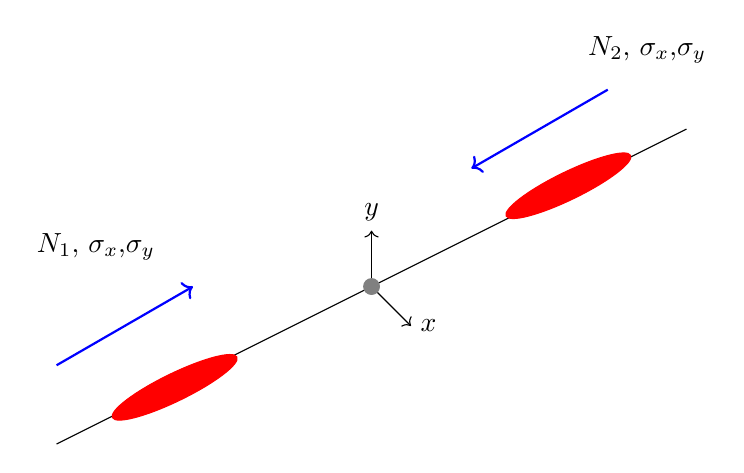
\begin{tikzpicture}
\draw (-4,-2) -- (4,2);
\draw[rotate around={26:(-2.5,-1.28)},fill,red] (-2.5,-1.28) ellipse (25pt and 5pt);
\draw[rotate around={26:(2.5,1.28)},fill,red] (2.5,1.28) ellipse (25pt and 5pt);
\draw[->,thick,blue] (-4,-1) -- +(30:2);
\draw[->,thick,blue] (3,2.5) -- +(210:2);
\node at (-3.5,0.5) {$N_1$, $\sigma_x$,$\sigma_y$};
\node at (3.5,3) {$N_2$, $\sigma_x$,$\sigma_y$};
\draw[->] (0,0) -- (0.5,-0.5) node[right] {$x$};
\draw[->] (0,0) -- (0,0.71) node[above] {$y$};
\draw[gray,fill] (0,0) circle [radius=0.1cm];
\end{tikzpicture}
\caption{Schematic view of colliding bunches with transverse dimensions $\sigma_x$ and $\sigma_y$. $N_1$,  $N_{2}$ are the number of particles per bunch.}
\end{figure}
%
%%%%%%%%%%%%%%%   END FIGURE  %%%%%%%%%%%%%%%%%%%%%%%%%%%%%%

\end{document}
